\section{Multiple distributions combined}
This subsection covers inputs that do not follow a specific distribution.
So instead of sampling from one distribution here instead the value is chosen from a set of distributions.
The used distributions were \textasciitilde$U(1,49999)$, \textasciitilde$B(10000,0.1)$, \textasciitilde$Geo(0.001)$, \textasciitilde$D^{1.25}_{50000}$.
Each distribution is chosen with probability $1/8$ and with remaining probability $1/2$ one value is drawn from every distribution and added together.
An input of this distribution is shown in Figure~\ref{fig:mixAndOverlDistExample}.
There are a lot of values close to 0 drawn from the powerlaw (and geometric) distribution.
The amount of values then decreases to around 50.
From then on the amount of generated numbers rises again until 100, the expected value of the binomial distribution.
After the spike caused by the binomial distribution the values look more uniform distributed until 1200 where they fall of again.
The higher the numbers get the less often they occur.

\begin{figure}[h]
      \caption{Distribution of a combined input with \textasciitilde$U(1,999)$, \textasciitilde$B(1000,0.1)$, \textasciitilde$Geo(0.01)$, \textasciitilde$D^{1.25}_{1000}$}
      \centering
      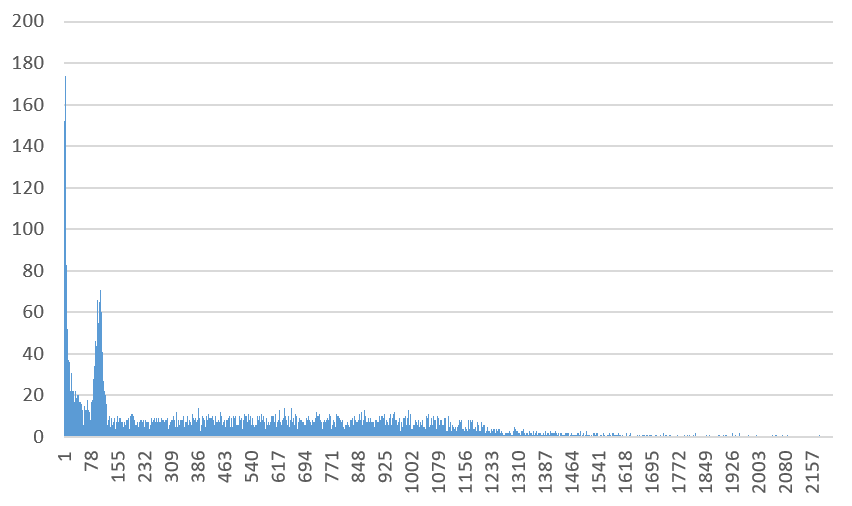
\includegraphics[width=0.7\textwidth]{figures/images/numberGenerator/mixedAndOverlapped.png}\label{fig:mixAndOverlDistExample}
\end{figure}

\subsection{RLS Comparison}
\makebox[\linewidth]{
\begin{tabular}{lp{3cm}p{6cm}p{6cm}}
\begin{tabular}[h]{cccccccc}
algo type&            \RLSN&     \RLSR&     \RLSR&     \RLSN&     \RLSR&     \RLSN&       RLS\\
algo param&             b=2&       s=3&       s=4&       b=3&       s=2&       b=4&         -\\
avg mut/change&       2.000&     1.996&     2.476&     3.000&     1.502&     4.000&     1.000\\
avg mut/step&         2.000&     2.000&     2.500&     3.000&     1.500&     4.000&     1.000\\
\hline
total avg count&     83,118&   104,748&   105,513&   112,223&   114,486&   121,927& 2,443,567\\
avg eval count&      83,118&   104,748&   105,513&   112,223&   114,486&   121,927&    45,834\\
max eval count&     778,110& 1,453,252&   898,974& 1,377,471&   915,268&   816,633&   485,275\\
min eval count&         197&       126&        45&       212&       271&       155&       128\\
\hline
fail ratio&           0.000&     0.000&     0.000&     0.000&     0.000&     0.000&     0.447\\
avg fail dif&             -&         -&         -&         -&         -&         -&         1\\
\end{tabular}
\end{tabular}
}


There is a clear preference of algorithms with higher probability to flip only one bit per step similar to the geometric distribution.
For geometric distributions all variants had a rather equal runtime but here the \RLSN[4] needs more than 100 time the iterations on average than the fastest RLS variant.
This type of input punishes the worse mutation operators more than geometric inputs but not as extreme as the equivalent to linear functions.
Here still every variant reaches an optimal solution in every case as opposed to the linear function equivalent.
For the geometric input only the RLS failed to reach an optimal value in every run but here it does not.
This leads to the RLS being the best RLS variants for this type of input in contrast to the geometric inputs.
\subsection{(1+1) EA Comparison}
\makebox[\linewidth]{
\begin{tabular}{lp{3cm}p{6cm}p{6cm}}
\begin{tabular}[h]{ccccccccc}
algo type&          (1+1) EA&   (1+1) EA&   (1+1) EA&   (1+1) EA&      (1+1) EA&   (1+1) EA&   (1+1) EA&   (1+1) EA\\
algo param&           3/n&     4/n&     2/n&     5/n&       -&    10/n&    50/n&   100/n\\
avg mut/change&     3.101&   3.968&   2.343&   4.859&   1.698&   9.732&  49.544&  99.494\\
avg mut/step&       2.999&   4.003&   2.002&   4.999&   1.001&   9.998&  49.998&  99.997\\
\hline
total avg count&      646&     701&     706&     857&   1,123&   1,508&   8,175&  15,485\\
avg eval count&       646&     701&     706&     857&   1,123&   1,508&   8,175&  15,485\\
max eval count&     5,346&   5,692&   3,415&   5,572&   7,001&  12,112&  52,831& 145,269\\
min eval count&        23&       4&      30&       9&      23&      14&      27&      69\\
\hline
fails&                  0&       0&       0&       0&       0&       0&       0&       0\\
fail ratio&         0.000&   0.000&   0.000&   0.000&   0.000&   0.000&   0.000&   0.000\\
avg fail dif&           -&       -&       -&       -&       -&       -&       -&       -\\
\end{tabular}
\end{tabular}
}


The results here are pretty similar to the results of the RLS.\
The lower the mutation rates the faster the algorithm reaches an optimal solution.
For $p_m\le10/n$ did not find an optimal solution in $10n\ln n$ steps in of the 10000 runs.
In other shorter experiments higher mutation rates reached an optimal solution less often.
The highest researched rate of $100/n$ even failed to reach the optimal solution in about 15 \% of the inputs.

\subsection{pmut Comparison}
\makebox[\linewidth]{
\scriptsize
\begin{tabular}{lp{3cm}p{6cm}p{6cm}}
\begin{tabular}[h]{m{2.5cm}m{0,40cm}m{0,40cm}m{0,40cm}m{0,40cm}m{0,40cm}m{0,40cm}m{0,40cm}m{0,40cm}m{0,40cm}m{0,40cm}m{0,40cm}m{0,40cm}m{0,40cm}m{0,40cm}m{0,40cm}m{0,40cm}m{0,40cm}m{0,40cm}}
\multicolumn{1}{c}{algo type}&\multicolumn{2}{c}{            pmut}&\multicolumn{2}{c}{     pmut}&\multicolumn{2}{c}{     pmut}&\multicolumn{2}{c}{     pmut}&\multicolumn{2}{c}{     pmut}&\multicolumn{2}{c}{     pmut}&\multicolumn{2}{c}{     pmut}&\multicolumn{2}{c}{     pmut}&\multicolumn{2}{c}{     pmut}\\
\multicolumn{1}{c}{algo param}&\multicolumn{2}{c}{           3.25}&\multicolumn{2}{c}{     3.00}&\multicolumn{2}{c}{     2.75}&\multicolumn{2}{c}{     2.50}&\multicolumn{2}{c}{     2.25}&\multicolumn{2}{c}{     2.00}&\multicolumn{2}{c}{     1.75}&\multicolumn{2}{c}{     1.50}&\multicolumn{2}{c}{     1.25}\\
\multicolumn{1}{c}{avg mut/change}&\multicolumn{2}{c}{      1.583}&\multicolumn{2}{c}{    1.737}&\multicolumn{2}{c}{    2.002}&\multicolumn{2}{c}{    2.423}&\multicolumn{2}{c}{    3.303}&\multicolumn{2}{c}{    5.830}&\multicolumn{2}{c}{   12.519}&\multicolumn{2}{c}{   30.910}&\multicolumn{2}{c}{   73.182}\\
\multicolumn{1}{c}{avg mut/step}&\multicolumn{2}{c}{        1.729}&\multicolumn{2}{c}{    1.934}&\multicolumn{2}{c}{    2.274}&\multicolumn{2}{c}{    2.895}&\multicolumn{2}{c}{    4.360}&\multicolumn{2}{c}{    8.452}&\multicolumn{2}{c}{   22.278}&\multicolumn{2}{c}{   70.532}&\multicolumn{2}{c}{  224.421}\\
\hline
\multicolumn{1}{c}{avg eval count}&\multicolumn{2}{c}{        540}&\multicolumn{2}{c}{      569}&\multicolumn{2}{c}{      594}&\multicolumn{2}{c}{      641}&\multicolumn{2}{c}{      712}&\multicolumn{2}{c}{      808}&\multicolumn{2}{c}{      967}&\multicolumn{2}{c}{    1,285}&\multicolumn{2}{c}{    2,081}\\
\multicolumn{1}{c}{max eval count}&\multicolumn{2}{c}{      3,110}&\multicolumn{2}{c}{    2,891}&\multicolumn{2}{c}{    3,504}&\multicolumn{2}{c}{    3,896}&\multicolumn{2}{c}{    5,152}&\multicolumn{2}{c}{    4,274}&\multicolumn{2}{c}{    5,610}&\multicolumn{2}{c}{    6,190}&\multicolumn{2}{c}{   14,984}\\
\multicolumn{1}{c}{min eval count}&\multicolumn{2}{c}{         22}&\multicolumn{2}{c}{        9}&\multicolumn{2}{c}{       36}&\multicolumn{2}{c}{       25}&\multicolumn{2}{c}{       28}&\multicolumn{2}{c}{       27}&\multicolumn{2}{c}{       27}&\multicolumn{2}{c}{       13}&\multicolumn{2}{c}{       33}\\
\hline
\multicolumn{1}{c}{fail ratio}&\multicolumn{2}{c}{          0.000}&\multicolumn{2}{c}{    0.000}&\multicolumn{2}{c}{    0.000}&\multicolumn{2}{c}{    0.000}&\multicolumn{2}{c}{    0.000}&\multicolumn{2}{c}{    0.000}&\multicolumn{2}{c}{    0.000}&\multicolumn{2}{c}{    0.000}&\multicolumn{2}{c}{    0.000}\\
\hline
\multicolumn{1}{c}{p-value}&&\multicolumn{2}{c}{0.0000}&\multicolumn{2}{c}{0.0000}&\multicolumn{2}{c}{0.0000}&\multicolumn{2}{c}{0.0000}&\multicolumn{2}{c}{0.0000}&\multicolumn{2}{c}{0.0000}&\multicolumn{2}{c}{0.0000}&\multicolumn{2}{c}{0.0000}\\
&&&&&&&&&&&&&&&&&&\end{tabular}
\end{tabular}
}


Here the results are similar again, but there are a few differences.
$\beta=2.5$ seems to perform better despite not being the highest value for $\beta$.
Here using a worse mutation rates are has less impact on the runtime in contrast to the geometric inputs where the penalty is higher.
Apart from that these inputs seem similar as every value of $\beta$ also reaches an optimal value in every run.

\subsection{Comparison of the best variants}
The ranking of the algorithm is the same as for the other inputs with a similar preference of low mutation rates.
The RLS variant has the best performance closely follow by $pmut_{3.25}$ and lastly be the standard (1+1) EA.\
For smaller values of $n$ the results are similar too.

\begin{tabular}[h]{ccccccccc}
fails in 1000 runs&20&50&100&500&1000&5000&10000&50000\\\hline
RLS&984&773&411&1&0&0&0&0\\
\RLSR[2]&890&241&14&0&0&0&0&0\\
(1+1) EA (1$/n$)&711&75&5&0&0&0&0&0\\
(1+1) EA (2$/n$)&541&14&0&0&0&0&0&0\\
pmut (3.0)&566&63&4&0&0&0&0&0\\
pmut (3.25)&587&63&7&0&0&0&0&0\\
\end{tabular}


The RLS variants perform the worst for at least $n\le 100$.
For this input it is also rather hard to find a perfect partition for $n\le50$.
For the lower values there were probability multiple inputs generated with mostly small values and an uneven number of large values.
Even if the amount of large numbers is even there might still be no perfect partition, hence no algorithm is able to reach one and the run is treated as a failed run.

\begin{tabular}[h]{ccccccccc}
avg&20&50&100&500&1000&5000&10000&50000\\\hline
RLS&32&79&153&579&950&1859&1922&1797\\
\RLSR[2]&391&2124&5005&4218&3530&2362&2160&2229\\
(1+1) EA (1$/n$)&22471&18343&12834&8342&6511&3815&3458&3371\\
(1+1) EA (2$/n$)&16360&9243&6452&4503&4020&3171&3141&3133\\
pmut (3.25)&23440&15929&9658&5644&4406&2434&2162&2172\\
pmut (3.0)&21901&14696&9186&5222&4150&2510&2208&2213\\
\end{tabular}


The inputs get easier to solve up until $n=5000$ and from then on get harder again with increasing input size.
The increase for larger input sizes is much smaller than the decrease for the small values.

\begin{tabular}[h]{ccccccccc}
total avg&20&50&100&500&1000&5000&10000&50000\\\hline
RLS&99470&93459&74385&3474&447&389&421&555\\
\RLSR[2]&96305&63088&19364&815&589&565&595&699\\
(1+1) EA (1$/n$)&89444&52886&21141&1410&869&850&875&1046\\
(1+1) EA (2$/n$)&79603&37214&14107&1302&992&942&957&1055\\
pmut (3.25)&84226&48403&18280&930&542&526&546&642\\
pmut (3.0)&82474&46286&17825&917&576&548&573&668\\
\end{tabular}



This type of inputs are best solved by the (1+1) EA with $p_m=2/n$ for $n\le100$.
Until $n<5000$ instead using $pmut_{3.0}$ or $pmut_{3.25}$ leads to a better running time.
After $n\ge5000$ the standard RLS becomes the best option and it seems like it stays that way for the remaining input sizes.
